\documentclass{article}
\usepackage{graphicx,fancyhdr,amsmath,amssymb,amsthm,subfig,url,hyperref}
\usepackage[margin=1in]{geometry}
\usepackage[brazilian]{babel}
\usepackage[utf8]{inputenc}
\usepackage{mathtools}
\usepackage{amssymb}
\usepackage{amsmath}
\usepackage{graphics}
\usepackage{fancyhdr}
\usepackage{lastpage}
\usepackage{subfigure}
\usepackage{listings}
\usepackage{color}                   % red, green, blue, yellow, cyan, magenta, black, white
\definecolor{mygreen}{RGB}{28,172,0} % color values Red, Green, Blue
\definecolor{mylilas}{RGB}{170,55,241}

\lstset{language=Matlab,%
    % basicstyle=\color{red},
    breaklines=true,%
    morekeywords={matlab2tikz},
    keywordstyle=\color{blue},%
    morekeywords=[2]{1}, keywordstyle=[2]{\color{black}},
    identifierstyle=\color{black},%
    stringstyle=\color{mylilas},
    commentstyle=\color{mygreen},%
    showstringspaces=false,             % without this there will be a symbol in the places where there is a space
    numbers=left,%
    numberstyle={\tiny \color{black}},  % size of the numbers
    numbersep=9pt,                      % this defines how far the numbers are from the text
    emph=[1]{for,end,break},emphstyle=[1]\color{red}, %some words to emphasise
    %emph=[2]{word1,word2}, emphstyle=[2]{style},    
}

%----------------------- Macros and Definitions --------------------------

%%% FILL THIS OUT
\newcommand{\studentname}{Bruno H. L. N. Peixoto}
\newcommand{\uspid}{7206666}
\newcommand{\uspmail}{bruno.peixoto@usp.br}
\newcommand{\esnumber}{1}
%%% END

\renewcommand{\theenumi}{\bf \Alph{enumi}}

\fancypagestyle{plain}{}
\pagestyle{fancy}
\fancyhf{}
\fancyhead[RO,LE]{\sffamily\bfseries\large Universidade de São Paulo}
\fancyhead[LO,RE]{\sffamily\bfseries\large PTC5611 Controle Digital de Sistemas Dinâmicos}
\cfoot{Página \thepage \hspace{1pt} de \pageref{LastPage}}	
\renewcommand{\headrulewidth}{1pt}

\graphicspath{{figures/}}

%-------------------------------- Title ----------------------------------

\title{Lista de exercícios \esnumber}
\author{\studentname \qquad Número USP: \uspid \qquad E-mail USP: \uspmail}

%--------------------------------- Text ----------------------------------

\begin{document}
\maketitle

O leitor pode encontrar todos os scripts utilizados neste documento em  \url{https://github.com/brunolnetto/Mestrado}.

\section*{Exercício 1}
\begin{enumerate}
\item %A

Por hipótese, a frequência de amostragem utilizada satisfaz o teorema de Nyquist \footnote{Essencialmente $\omega_s \geq 2\omega_0$, onde $\omega_s$ corresponde a frequência de amostragem e $\omega_0$ a máxima frequência do sinal amostrado.}. Como $t = kT_s = \frac{k}{f_s}$, temos que.

\begin{equation}
\label{eq:ex1a}
x[k] = cos(k \frac{\omega}{f_s})  \stackrel{!}{=} cos(k \alpha) \Longleftrightarrow \alpha = \frac{\omega}{f_s}
\end{equation}

Assim, $\omega = 250\pi \frac{rad}{s}$. A imagem (\ref{fig:ex1}) apresenta o sinal original e o amostrado.

\begin{figure}[!h]
	\center
	\includegraphics[width=0.6\textwidth]{./images/ex1a.eps}
	\caption{Curva original e série amostrada}
	\label{fig:ex1}
\end{figure}

\item %B
Pela equação (\ref{eq:ex1a}), conclui-se que $f_s = 12$ $kHz$. Dada frequência do sistema de $4000\pi \frac{rad}{s}$, pelo teorema de Nyquist $\omega_s \stackrel{!}{>} 8000\pi \frac{rad}{s} \approx 24000 \frac{rad}{s}$. Devido à violação, não é possível reconstruir o sinal por meio de um filtro passa-baixas ideal. 

\item %C
Para sinais senoidais amostrados com frequência $f_s$, tem-se que, para uma mesma série $x[n] = cos(\alpha n)$, os possíveis sinais advindos deste são $x(t) = cos(2 \pi (f_0 + f_s)t) \mbox{, } k \in \mathbb{N} \mbox{, } \omega = 2 \pi f$. Por (\ref{eq:ex1a}), tem-se que $\omega_0 = \frac{5\pi}{4} \frac{rad}{s}$. Assim, dois possíveis sinais para a série fornecida são $x_1(t) = cos(\frac{5\pi}{4} t )$ e $x_2(t) = cos(\frac{85\pi}{4} t)$.

\item %D

Para o caso presente na figura (\ref{fig:ex1d1}), o sinal reconstruido é distorcido. Em contrapartida, por respeitar o critério de Nyquist, o sinal reconstruido é o mesmo do sinal original, presente na figura (\ref{fig:ex1d2}).

\begin{figure}[!h]
    \centering
    \includegraphics[width=0.6\textwidth]{./images/ex1d1.eps}
    \caption{Espectro de Fourier do sinal original, amostrado com $\omega_s = \omega_N$, e reconstruído por  filtro com $\omega_f = \omega_N$}
    \label{fig:ex1d1}
\end{figure}%

\begin{figure}![!h]
    \centering
    \includegraphics[width=0.6\textwidth]{./images/ex1d2.eps}
    \caption{Espectro em frequência do sinal original, amostrado com $\omega_s = 3 \, \omega_N$ e reconstruído por  filtro com $\omega_f = \frac{\omega_s}{2}$}
    \label{fig:ex1d2}
\end{figure}

\end{enumerate}

\section*{Exercício 2}

\begin{enumerate}
\item %A

As demonstrações estão enunciadas abaixo:

\begin{itemize}
	\item $Z\{\sum_{i=0}^{n}x[i] \} = \frac{1}{1-z^{-1}}X(z)$
	
	\begin{equation}
	\begin{split}
	Z\{\sum_{i=0}^{n}x[i] \} & = \sum_{n=0}^{\infty} z^{-n} \sum_{i=0}^{n} x[i] \\
	& = x[0] + z^{-1} \sum_{i=0}^{1} x[i] + z^{-2} \sum_{i=0}^{2} x[i] + \cdots \\
	& = x[0] \sum_{i=0}^{\infty} z^{-i} + x[1] \sum_{i=1}^{\infty} z^{-i} + \cdots + x[k] 
	\underbrace{\sum_{i=k}^{\infty} z^{-i}}_{\frac{z^{-k}}{1 - z^{-1}}} + \cdots\\
	& = x[0] \frac{1}{1 - z^{-1}} + x[1] \frac{z^{-1}}{1 - z^{-1}} + \cdots \\
	& = \frac{1}{1 - z^{-1}} \underbrace{\sum_{i=0}^{\infty} x[i].z^{-i}}_{\coloneqq X(z)}
	\end{split}
	\end{equation}

	\begin{equation}
	\therefore Z\{\sum_{i=0}^{n}x[i] \} = \frac{1}{1-z^{-1}}.X(z) \hspace{10pt} \blacksquare
	\end{equation}
	
	\item $Z\{\sum_{i=0}^{n}x[i-1] \} = \frac{z^{-1}}{1-z^{-1}}X(z)$

	\begin{equation}
	\begin{split}
	Z\{\sum_{i=0}^{n}x[i] \} & = \sum_{n=0}^{\infty} z^{-n} \sum_{i=0}^{n} x[i-1] \\
	& = x[-1] + z^{-1} \sum_{i=0}^{1} x[i-1] + z^{-2} \sum_{i=0}^{2} x[i-1] + \cdots \\
	& = \underbrace{x[-1]}_{\coloneqq 0} \sum_{i=0}^{\infty} z^{-i} + x[0] \sum_{i=1}^{\infty} z^{-i} + \cdots \\
	& = x[0] \frac{z^{-1}}{1 - z^{-1}} + x[1] \frac{z^{-2}}{1 - z^{-1}} + \cdots \\
	& = \frac{z^{-1}}{1 - z^{-1}} \underbrace{\sum_{i=0}^{\infty} x[i].z^{-i}}_{\coloneqq X(z)}
	\end{split}
	\end{equation}

	\begin{equation}
	\therefore Z\{\sum_{i=0}^{n}x[i-1] \} = \frac{z^{-1}}{1-z^{-1}}.X(z) \hspace{10pt} \blacksquare
	\end{equation}

	\item $\lim\limits_{z \rightarrow 1} X(z) = \sum_{i=0}^{\infty}x[i]$

	\begin{equation}
	\lim\limits_{z \rightarrow 1} X(z) & = \lim\limits_{z \rightarrow 1} \sum_{i=0}^{\infty} x[i].z^{-i} = \sum_{i=0}^{\infty} x[i]
	\end{equation}
	
	\begin{equation}
	\begin{split}
	\therefore \lim\limits_{z \rightarrow 1} X(z) = \sum_{i=0}^{\infty}x[i] \hspace{10pt} \blacksquare
	\end{split}
	\end{equation}
	
\end{itemize}

\item\label{item:ex2b} %B
Dada função $x_1(t) = \frac{1}{a} \left( 1 - e^{-at} \right)$, por definição, tem-se que:

	\begin{equation}
	\begin{split}
	Z\{x_1(t)\} = X_1(z) & = \sum_{i=0}^{\infty} x_1(i Ts).z^{-i} \\
	& = \frac{1}{a} \sum_{i=0}^{\infty} \left( 1 - e^{-a T_s i} \right)z^{-i} \\
	& = \frac{1}{a} \sum_{i=0}^{\infty} z^{-i} - \frac{1}{a} \sum_{i=0}^{\infty} \underbrace{e^{-a T_s i}.z^{-i}}_{(z.e^{aT_s})^{-i}}
	\end{split}
	\end{equation}

Se $|z| > 1$ e $|z| > e^{aT_s}$, então:
	
	\begin{equation}
	\begin{split}
	\frac{1}{a} \sum_{i=0}^{\infty} z^{-i} - \frac{1}{a} \sum_{i=0}^{\infty} e^{-a T_s i}.z^{-i} & = \frac{1}{a} (\frac{1}{1-z^ {-1}} - \frac{1}{1-e^{-aT_s} z^ {-1}}) \\
	& = \frac{1}{a} \frac{(1 - e^{-aT_s})z^{-1}}{(1-z^{-1})(1-e^{-aT_s} z^ {-1})}
	\end{split}
	\end{equation}
	
Portanto
	
	\begin{equation}
	X_1(z) = \frac{1}{a}  \frac{(1 - e^{-aT_s})z^{-1}}{(1-z^{-1})(1-e^{-aT_s} z^ {-1})}
	\end{equation}

De mesma forma, dada função $x_2(t) = $t^2 e^{-a t}$, por definição tem-se que:

	\begin{equation}
	\begin{split}
	Z\{x_2(t)\} = X_2(z) & = \sum_{i=0}^{\infty} x_2(i Ts).z^{-i} \\
	& = \sum_{i=0}^{\infty} \left( i^2 T_s^2 e^{-a T_s i} z^{-i} \right) \\
	& = \sum_{i=0}^{\infty} T_s^2 i^2 e^{-a T_s i} z^{-i}
	\end{split}
	\end{equation}
	
Por meio da propriedade da transformada $\mathcal{Z}\{n X[n]\} \coloneqq -z \frac{d}{dz} X(z)$, segue

\begin{subequations}
\begin{equation}
x[n] = e^{-an} & \rightarrow -z \frac{d}{dz} \mathcal{Z}\{e^{-an}\} = \mathcal{Z}\{n e^{-an}\} \mbox{, } n = T_s i \mbox{, } i \in \mathbb{N}
\end{equation}
\begin{equation}
x[n] = n e^{-an} & \rightarrow -z \frac{d}{dz} \mathcal{Z}\{n e^{-an}\}} = \mathcal{Z}\{n^2 e^{-an}\} \mbox{, } n = T_s \mbox{, } i \in \mathbb{N}
\end{equation}
\end{subequations}

Logo

    \begin{equation}
    \begin{split}
    \mathcal{Z}\{e^{-an}\} & = \frac{1}{1 - e^{-a T_s} z^{-1}} \Rightarrow \\
    \frac{d}{dz} \mathcal{Z}\{e^{-an}\} & = - e^{-a T_s} \frac{z^{-2}}{(1 - e^{-a T_s} z^{-1})^2} \\
    \mathcal{Z}\{n e^{-an}\} \coloneqq -z \frac{d}{dz} \mathcal{Z}\{e^{-an}\} & = e^{-a T_s} \frac{z^{-1}}{(1 - e^{-a T_s} z^{-1})^2}
    \end{split}
    \end{equation}

e

    \begin{equation}
    \begin{split}
    \mathcal{Z}\{n e^{-an}\} & = e^{-a T_s} \frac{z^{-1}}{(1 - e^{-a T_s} z^{-1})^2} \Rightarrow \\ \frac{d}{dz} \mathcal{Z}\{n e^{-an}\} & = e^{- a T_s} \frac{z^{-2}(1 - e^{-a T_s} z^-1)^2 - 2(1 - e^{-a T_s} z^{-1}) e^{-a T_s} z^{-2}}{(1 - e^{-a T_s} z^{-1})^3} \\ 
    & = - e^{-a T_s} \frac{z^{-2} (1 + e^{-a T_s} z^{-1})}{(1 - e^{- a T_s} z^-1)^3}
    \end{split}
    \end{equation}

Portanto 

\begin{equation}
    \mathcal{Z}\{n^2 e^{-a n}\} \coloneqq -z \frac{d}{dz} \mathcal{Z}\{n e^{-a n}\} & = e^{-a T_s} \frac{z^{-1}(1 + e^{-a T_s} z^{-1})}{(1 - e^{-a T_s} z^{-1})}
\end{equation}

\item %C
Por definição, a equação das diferenças é da forma

\begin{equation}
\sum_{i=0}^{m} b_i y[n-i] = \sum_{i=0}^{n} a_i x[n-i]
\end{equation}

com parâmetros dados por $m = n = 3$ e $a_i, b_i$, $i = 1, 2, 3$ dados por $a_0 = 1$, $a_1 = -0.9737$, $a_2 = 0.8101$, $a_3 = 0.8151$, $a_1 = -0.0515$, $b_0 = 0.4108$, $b_1 = -1.0094$, $b_2 = 1.0094$ e $b_3 = 0.4108$. A função de transferência equivalente é

\begin{equation}
G(z) = \frac{Y(Z)}{X(z)} = \frac{\sum_{i=0}^{m} b_{i} z^{-i}}{\sum_{i=0}^{n} a_{i} z^{-i}} = \frac{\sum_{i=0}^{m} b_{m-i} z^{i}}{\sum_{i=0}^{n} a_{n-i} z^{i}}
\end{equation}

Assim, as raízes do numerador e denominador, nomeadamente zeros e pólos, são respectivamente $z = \{1.38 \pm 1.18 i, -0.3\}$ e $p = \{0.45 \pm 0.74i, 0.068\}$.

\end{enumerate}

\section*{Exercício 3}
Dado sinal discreto $a[n]$ resultado da primeira soma à esquerda no diagrama de blocos, temos que:

\begin{equation}
\label{eq:ex31}
A(z) = 2 X(z) - 2 z^{-1} X(z) 0.3 - 0.5 z^{-2} Y(z)
\end{equation}

De mesma forma,

\begin{equation}
\label{eq:ex32}
Y(z) = -z^2 X(z) + A(z) - z^{-1} Y(z)
\end{equation}

Substituindo-se (\ref{eq:ex31}) em (\ref{eq:ex32}), obtém-se:

\begin{equation}
\begin{split}
-z^{-2} X(z) + 2 X(z) - 0.6  z^{-1} X(z) - 0.5 z^{-2} Y(z) - z^{-1} Y(z) \\
\frac{Y(z)}{X(z)} = \frac{- z^{-2} - 0.6 z^{-1} + 2}{0.5 z^-2 + z^{-1} + 1} = \frac{2 z^{2} - 0.6 z - 1}{z^2 + z + 0.5}
\end{split}
\end{equation}

Os pólos do sistema são estáveis pois $z = \pm\frac{\sqrt{2}}{2}$ encontram-se no interior do circulo unitário, região estável em tempo discreto.

A imagem (\ref{fig:ex3sim}) refere-se à simulação do diagrama fornecido e a função de transferência encontrada e a imagem (\ref{fig:ex3diag}) referem-se ao diagrama utilizado no MatLab/Simulink. Perceba que, em (\ref{fig:ex3sim}), ambos os sinais sobrepõem-se nos instantes múltiplos do tempo de amostragem. 

\begin{figure}[!h]
	\center
	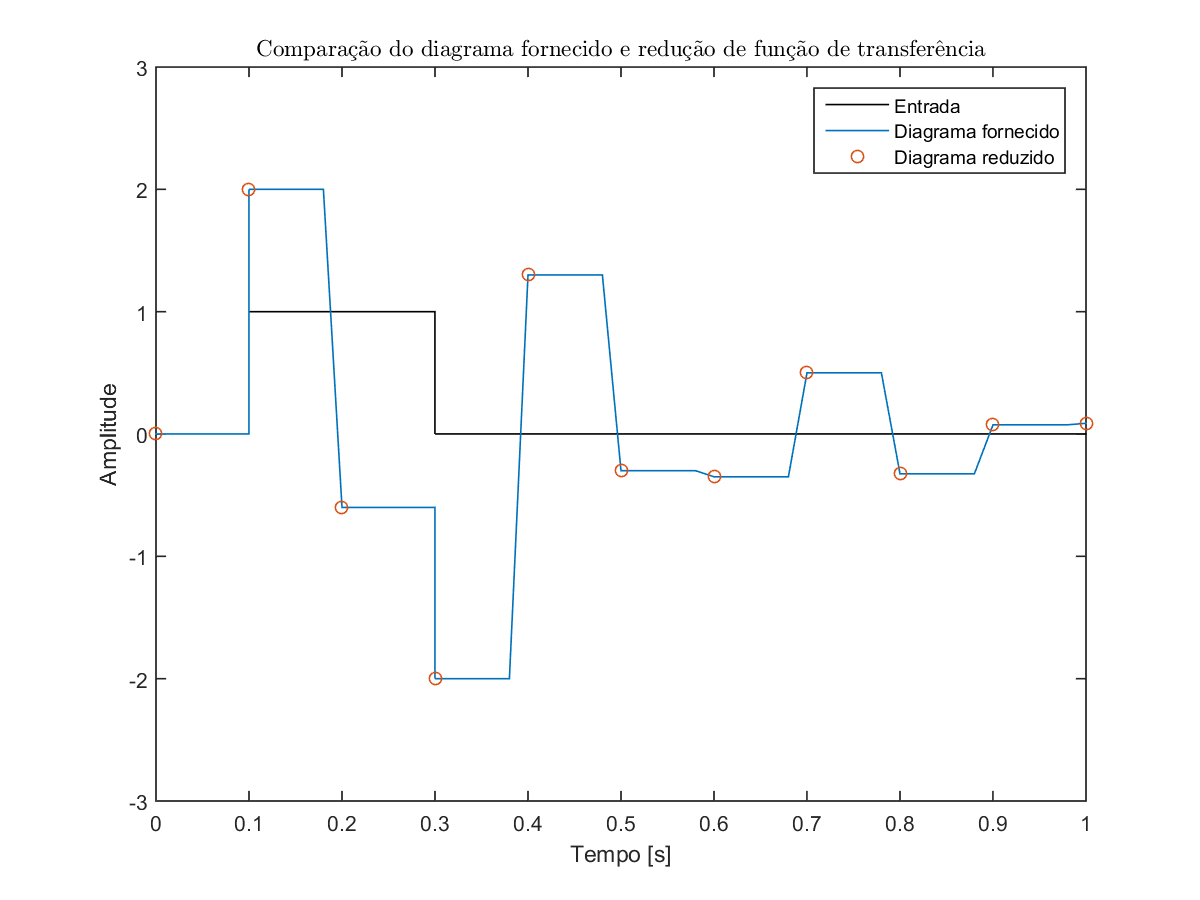
\includegraphics[width=\textwidth]{./images/ex31.png}
	\caption{Entrada do sistema amostrado e saídas do diagrama amostrado e função de transferência equivalente}
	\label{fig:ex3sim}
\end{figure}

\begin{figure}[!h]
	\center
	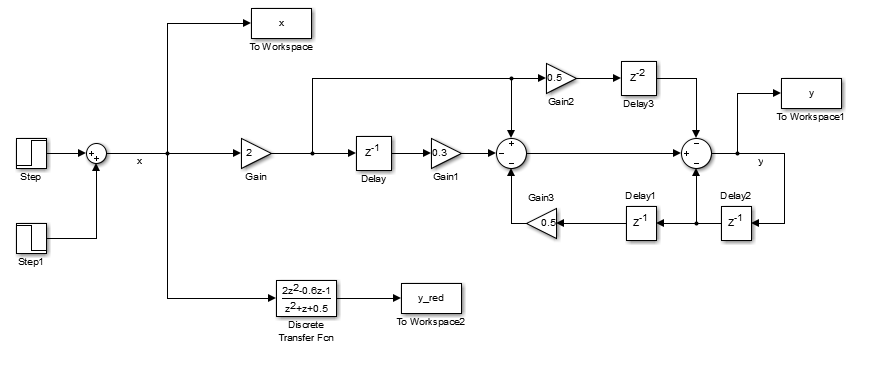
\includegraphics[width=\textwidth]{./images/ex3simulink.png}
	\caption{Diagrama de blocos do sistema simulado}
	\label{fig:ex3diag}
\end{figure}

\section*{Exercício 4}

A conversão sem aproximação do espaço contínuo para discreto com mantenedor de ordem zero (ZOH) satisfaz a seguinte equação:

\begin{equation}
G(z) \coloneqq (1-z^{-1}) \mathcal{Z}\left\{\mathcal{L}^{-1}\left\{\frac{G(s)}{s}\right\}\right\}
\end{equation}

Desta forma

\begin{equation}
\label{eq:ex41}
\frac{G(s)}{s} = H(s) = \frac{K}{s(s+a)}
\end{equation}

Pelo método de expansão de frações parciais, a equação (\ref{eq:ex41}) apresenta a seguinte forma

\begin{equation}
H(s) = \frac{A}{s} + \frac{B}{(s+a)} 
\end{equation}

Onde 

\begin{equation}
A = H(s) s \bigg\rvert_{s=0} = \frac{K}{a} \mbox{ e } B = H(s) (s+a)\bigg\rvert_{s=-a} = -\frac{K}{a}
\end{equation}

Logo

\begin{equation}
H(s) = \frac{K}{a} \left( \frac{1}{s} - \frac{1}{s+a} \right)
\end{equation}

A função de transferência acima exceto ao fator de escala $j$ foi obtida no item (\ref{item:ex2b}). Desta forma

\begin{equation}
\label{eq:lapinv}
\mathcal{L}^{-1}\left\{\frac{G(s)}{s}\right\} = \frac{K}{a}\sigma(t)\left(1+e^{-at}\right)
\end{equation}

Portanto, a função $\mathcal{Z}$ da função (\ref{eq:lapinv}) é dada por

\begin{equation}
G(z) = \frac{K}{a} \frac{(1 - e^{-aT_s}z^{-1})}{(1-z^{-1})(1 - e^{-aT_s}z^{-1})}
\end{equation}

Por fim, por meio da função de transefrência de uma malha fechada \footnote{A equação em malha fechada de um sistema em tempo discreto ou contínuo é dado pela equação $G_{MF}(z) = \frac{G(z)}{1+G(z)}$}, após certa manipulação algébrica é dada por:

\begin{equation}
G_{MF}(z) = K' \frac{z}{z+b}
\end{equation}

onde $K' = \frac{K}{a} (1-e^{-aT_s}) \mbox{ e } b = \left[\left[(1 + \frac{k}{a})\right]e^(-aT_s) - \frac{k}{a} \right] $.

\section*{Exercício 5} Dados: Ts = 0,1 s

\begin{enumerate}
\item % A

\begin{equation}
\begin{split}
s = \frac{z - 1}{T_s} \therefore X(z) = \frac{\frac{z+1}{T_s} + 1}{\frac{z+1}{T_s} + 10} = \frac{z - (1-T_s)}{z - (1-10T_s)} = \frac{z - 0.9}{z} 
\end{split}
\end{equation}

\item % B

\begin{equation}
\begin{split}
s = \frac{z - 1}{T_s z} \therefore X(z) = \frac{\frac{z-1}{T_s z} + 1}{\frac{z-1}{T_s z} + 10} = \frac{(1+T_s) z - 1}{(1 + 10T_s) z + 1} = 0.45 \frac{z - 1.1}{z - 0.5}
\end{split}
\end{equation}

\item % C

\begin{equation}
\begin{split}
s = \frac{2}{T_s} \frac{z - 1}{z+1} \therefore X(z) = \frac{\frac{2}{T_s} \frac{z-1}{z+1} + 1}{\frac{2}{T_s} \frac{z-1}{z+1} + 10} = \frac{(2+T_s)z + (T_s - 2)}{(2 + 10T_s) z + (10 T_s - 2)} = \frac{2.1z - 1.9}{3z - 1} = 0.7\frac{z-0.63}{z-0.33}
\end{split}
\end{equation}

\item % D
Dados: $\omega_c = 3 \frac{rad}{s}$

\begin{equation}
s = \frac{\omega_c}{\tan{\frac{\omega_c T_s}{2}}} \frac{z-1}{z+1} \therefore X(z) = \frac{\frac{\omega_c}{\tan(\frac{\omega_c T_s}{2})} \frac{z-1}{z+1} + 1}{\frac{\omega_c}{\tan(\frac{\omega_c T_s}{2})} \frac{z-1}{z+1} + 10} = \frac{(\tan{\frac{\omega_c T_s}{2}} + \omega_c) z + (\tan{\frac{\omega_c T_s}{2}} - \omega_c)}{(10 \tan{\frac{\omega_c T_s}{2}} + \omega_c) z + (10 \tan{\frac{\omega_c T_s}{2}} - \omega_c)} 
\end{equation}

Como $\frac{\omega_c T_s}{2} \ll 1$ e $\tan{\theta} \approx \theta$, então $\tan{\frac{\omega_c T_s}{2}} \approx \frac{\omega_c T_s}{2}$. Assim

\begin{equation}
X(z) = \frac{3.15\ - 2.85}{4.15z - 1.5} = 0.76 \frac{z - 0.9}{z - 0.36}
\end{equation}

\item % E
Todo pólo e zero da planta pode ser mapeado diretamente para o espaço $\mathcal{Z}$ pela relação $z = e^{s T_s}$. O ganho da função em regime estacionário devem ser ambos em espaço discreto quanto contínuo iguais.

\begin{equation}
\lim\limits_{z \rightarrow 1} X(z) \stackrel{!}{=} \lim\limits_{s \rightarrow 0} X(s) 
\end{equation} 

Desta forma.

\begin{equation*}
\begin{split}
K_z \frac{1 - e^{-Ts}}{1 - e^{-10Ts}} = \frac{1}{10} \Rightarrow K_z = 10 \frac{1 - e^{-10T_s}}{1 - e^{-T_s}} \approx 1.59
\end{split}
\end{equation*}

Portanto

\begin{equation}
X(z) = 1.59 \frac{z - 0.9}{z - 0.37}
\end{equation}

\end{enumerate}

\section*{Exercício 6}
Para que a função de transferência em malha fechada do sistema seja de segunda ordem, o controlador deve ser proporcional.O polinômio característico da função de transferência é:

\begin{equation}
P(s) = s^2 + 7s + k \stackrel{!}{=} s^2 + 2 \zeta \omega_n + \omega_n^2
\end{equation}

O tempo de subida é dada pela identidade:

\begin{equation}
\label{eq:sobressinal}
t^{0\% - 100\%}_{r}(\omega_n, \zeta) = \frac{\pi - \theta(\zeta)}{\omega_d(\omega_n, \zeta)} \mbox{, com } \theta(\zeta) = \tan^{-1}\frac{\sqrt{1 - \zeta^2}}{\zeta} \mbox{ e } \omega_d(\omega_n, \zeta) = \omega_n \sqrt{1-\zeta^2}
\end{equation}

De mesma forma, o sobressinal é dado por:

\begin{equation}
\label{eq:sobressinal}
M(\zeta) = e^{-\pi \frac{\zeta}{\sqrt{1-\zeta^2}}}
\end{equation}

Como (\ref{eq:sobressinal}) é bijetora, $\exists g(M) = \zeta \mbox{, } g: M \rightarrow g(M) \mbox{, } M \circ g (M) = M$. De fato $g(M) = \sqrt{\frac{\log^2{M}}{\pi^2 - \log^2{M}}}$. Assim, $\zeta \approx 0.672$. De mesma forma, para $\zeta$ fixo, analogamente, $\exists h(t_r) = \zeta\mbox{, }h: t_r \rightarrow h(t_r)\mbox{, } t_r(\zeta) \circ h = t_r$. De fato, $g(t_r) = \frac{\pi - \theta}{\omega_d(\zeta, t_r)}$. Assim, para $\zeta = 0.672$, então $\omega_n = 4.46$.  Como $\omega_n^2 = k$, então $k = 19.96$.

\section*{Exercício 7}

A função de transferência de um controlador PID é dada por:

\begin{equation}
C(s) = K_p\left(1 + \frac{1}{T_i s} + T_d s\right) = K \, \frac{s^2 + b s + c}{s}
\end{equation}

Os quais $K = K_p T_d $, $b = \frac{1}{T_d}$ e $c = \frac{1}{T_i T_d}$. Com auxílio da equação do exercício (\ref{ex:ex8}), conclui-se que, por meio da transformação para trás, a função de transferência de um controlador PID segue

\begin{equation}
G(s) = \frac{}{}
\end{equation}

Em caso geral, a fim da conversão de uma função de transferência $G(z)$ em sua respectiva função de diferenças e assim ação de controle do instante atual $kT_s$, seja essa em sua forma matricial

\begin{equation}
G(z) = \frac{b^T \textbf{z}_m}{a^T \textbf{z}_n}    
\label{eq:Gz}
\end{equation}

Os quais $a \in \mathbb{R}^n$, $b \in \mathbb{R}^m$ e $\mathcal{Z}_k = \left[z^k, \cdots, 1\right]^T$. Após manipulação algébrica, $\textbf{z}_p = z^p \, \textbf{v}_p$, $\textbf{v}_p = [1, \cdots, z^{-p}]$. A fim de manter a convenção para $z^{-1}$ dada por $\textbf{w}_p =  [z^{-p}, \cdots, 1]$, $\textbf{w}_p = \textbf{J}_p^{-1} \textbf{v}_p$ com $\textbf{J}_p$ a matriz de permuta, descrita em (\ref{eq:exchange}).

\begin{equation}
\textbf{J}_p = 
\begin{bmatrix}
0&\cdots&1\\
\vdots & \ddots & \vdots\\
1&\cdots&0\\
\end{bmatrix}
\label{eq:exchange}
\end{equation}

\begin{equation}
G(z) & = \frac{\textbf{b}^T \textbf{J}^{-1}_{m+1} \textbf{w}_m}{\textbf{a}^T \textbf{J}^{-1}_{n+1} \textbf{w}_n} & \coloneqq \frac{\textbf{b'}^T \textbf{w}_{m'+1}}{\textbf{a'}^T \textbf{w}_{n'+1}} 
\label{eq:Gz}
\end{equation}

Os parâmetros $\textbf{a'}$ e $\textbf{b'}$ acima estão a seguir

\begin{equation}
\textbf{a'} = [\textbf{0}_{m-n, 1}, \textbf{a}^T \textbf{J}_{n+1}]^T] & n < m
\label{eq:a}
\end{equation}

\begin{equation}
\textbf{b'} = [\textbf{0}_{m-n, 1}, \textbf{b}^T \textbf{J}_{m+1}]^T, & n \geq m
\label{eq:b}
\end{equation}

Ademais, $n' = \dim(\textbf{a'})$ e $m' = \dim(\textbf{b'})$. A equação de diferenças de (\ref{eq:Gz}), é, por definição:

\begin{equation}
G(z) = \frac{Y(z^{-1})}{U(z^{-1})} = \frac{\textbf{b}^T \textbf{w}_{m+1}}{\textbf{a}^T \textbf{w}_{n+1}} \Rightarrow a^T \textbf{y}[k] = b^T \textbf{u}[k]
\label{eq:eqdiferencas}
\end{equation}

Por inspeção, os parâmetros da equação de diferenças seguem de (\ref{eq:a}) e (\ref{eq:b}). O vetor $\textbf{u}$ pode ser escrito como $\textbf{u}[k] = \textbf{I}_{m' + 1} - \Delta_{m', m'} \textbf{u}[k] + \Delta_{m', m'} \textbf{u}[k]$. Assim

\begin{equation}
\textbf{b'}^T \underbrace{\Delta_{m' + 1 \times m' + 1} \textbf{u}[k]}_{\textbf{e}_{m'+1}} = \textbf{a'} \textbf{y}[k] - \textbf{b'}^T (\textbf{m} - \Delta_{m' + 1 \times m' + 1}) \textbf{u}[k]
 \end{equation}

Portanto

\begin{equation}
u[k] = (\textbf{b'}^T \textbf{e}_{m' + 1})^{-1}(\textbf{a'}^T \textbf{y}[k] - \textbf{b'}^T (\textbf{I}_{m' + 1} - \Delta_{m' + 1 \times m' + 1}) \textbf{u}[k])
\end{equation}

Para o caso em estudo, $n = 2$ e $m = 1$. Logo, $n < m$ e $\textbf{a'} = [\textbf{0}_{m-n, 1}, \textbf{a}^T \textbf{J}^{-1}_{n+1}]^T]$

\begin{enumerate}
\end{enumerate}

\section*{Exercício 7}

\section*{Exercício 8}
\label{ex:ex8}

O objetivo é encontrar $G(z)$ dada transformação $s = F(z)$. Em geral, as transformações aplicadas em engenharia respeitam a relação $s = \frac{c^T \mathcal{Z}}{d^T \mathcal{Z}}$, $c, d \in \mathbb{R}^2$, $\mathcal{Z}^T = [z, 1] $. Para a função de transferência dada por $G(s) = \frac{b^T \mathcal{S}_m}{a^T \mathcal{S}_n}$, tal que $\mathcal{S}_k^T = [s^k, \cdots, 1]  \, \in \, \mathbb{R}^{k+1}$, $m = \dim(b)$ e $n = \dim(a)$ e $s \in \mathbb{C}$, segue

\begin{equation}
s^i = \frac{c^T \mathcal{Z} \, c^T \, \mathcal{Z} \, \cdots \, c^T \, \mathcal{Z}}{d^T \, \mathcal{Z} \, d^T \, \mathcal{Z} \, \cdots d^T \, \mathcal{Z}} \, i \in \mathbb{N}
\label{eq:sexpi}
\end{equation}

Por definição, $a b^T = M \,\, M \in \mathbb{R}^{2x2}$ e $M = W \Lambda V$, com $V$ a matriz de autovetores de $M$, $\Lamba$ a matriz de autovalores de $M$ e $W = V^{-1}$ e $f(M) = W f(\Lambda) V$. Em especial, $M^i = W \Lambda^i V$. Assim, a equação (\ref{eq:sexpi}) reduz-se a:

\begin{equation}
s^i = \frac{c^T W_c \Lambda_c^{i-1} V_c \mathcal{Z}}{d^T W_d \Lambda_d^{i-1} V_d \mathcal{Z}}
\end{equation}

Perceba que o expoente de $\Lambda$ deve ser $i - 1$. Assim, 

\begin{equation}
\mathcal{S}_k^T = \left[\frac{c^T W_c \Lambda_c^{k-1} V_c \mathcal{Z}}{d^T W_d \Lambda_d^i V_d \mathcal{Z}}, \cdots, \frac{c^T W_c \Lambda_c^{-1} V_c \mathcal{Z}}{d^T W_d \Lambda_d^i V_d \mathcal{Z}}\right]
\end{equation}
$\mathcal{S}_k$ 

Deste modo, a função convertida pela função de transformação $s = \frac{c^T \mathcal{Z}}{d^T \mathcal{Z}}$ é dada por

\begin{equation}
G(z) = \frac{b^T \mathcal{S}_m}{c^t \mathcal{S}_n}    
\end{equation}

\begin{equation}
\mathcal{S}_k^T = [\frac{c^T W_c \Lambda_c^{k-1} V_c \mathcal{Z}}{d^T W_d \Lambda_d^i V_d \mathcal{Z}}, \cdots, \frac{c^T W_c \Lambda_c^{-1} V_c \mathcal{Z}}{d^T W_d \Lambda_d^i V_d \mathcal{Z}}]
\end{equation}

A implementação em MatLab encontra-se no apêndice 

\section*{Exercício 9}


\end{document}
